\newcommand{\tbontype}{\textsc{tbon}\textunderscore \textsc{tc}\textunderscore  \textsc{type}}
\newcommand{\tbonclasstype}{\textsc{tbon}\textunderscore \textsc{tc}\textunderscore \textsc{class}\textunderscore  \textsc{type}}
\newcommand{\tbonclustertype}{\textsc{tbon}\textunderscore \textsc{tc}\textunderscore \textsc{cluster}\textunderscore  \textsc{type}}
\newcommand{\tbonfeature}{\textsc{tbon}\textunderscore \textsc{tc}\textunderscore \textsc{feature}}
\newcommand{\tbongeneric}{\textsc{tbon}\textunderscore \textsc{tc}\textunderscore \textsc{generic}}

\section{Type Checker}
\subsection{Parsing and Lexing}
\begin{figure}[H]
    \centerline{\scalebox{0.75}{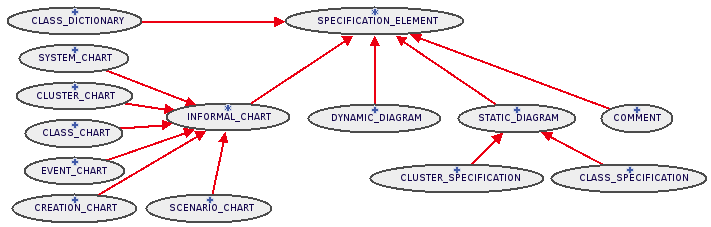
\includegraphics{images/mog2.png}}}
    \caption[MOG hierarchy]{First three levels of the inheritance hierarchy of the MOG}
    \label{fig:mog-hierarchy}
\end{figure}

%explain what a bon element is

\subsection{Building the Context}
\label{implementation-context-class-structure}
The type contexts for type checking of both informal and formal specifications are built using a hierarchy of types. This hierarchy is shown in figure \ref{fig:context-classes}.
\begin{figure}[H]
    \centerline{\scalebox{0.6}{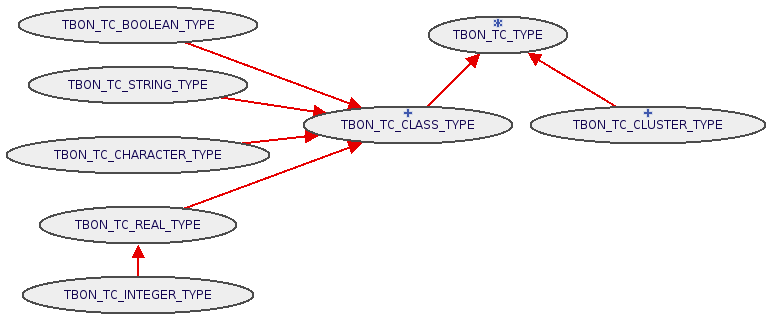
\includegraphics{images/context_classes3.png}}}
    \caption[Context classes]{Hierarchy of classes used to build the type contexts}
    \label{fig:context-classes}
\end{figure}
A context, be it informal or formal, is built as a set of instances of \tbonclasstype   and \tbonclustertype   (declared as a set of \tbontype ). Due to the naming restrictions discussed in section \ref{design-type-names}, classes and clusters are kept in the same context for convenience and easy detection of name clashes. At any time, the instances in the context represent the defined types currently known at that point.
\paragraph{} Mapping from classes to features (in formal specifications) happens through association with a set of \tbonfeature . An instance of \tbonclasstype  is never associated with an undefined feature, but can be associated with an inconsistent or ill-typed feature (elaboration on this is found in section \ref{implementation-unresolved-elements}). Accordingly, the type of a feature is merely an association to an instance of \tbonclasstype .
\paragraph{} Analogous to the mapping from classes to features, mapping from classes to generics is done through association with a sequence of \tbongeneric  (generics cannot be stored in a set, as the order of the type parameters matters). A generic type has both a bounding and an actual class type. The association between these is explained in section \ref{implementation-generics}.

%Transitional paragraph about phases and contexts here
\paragraph{}
Types defined in the abstract syntax is primarily added to the context in the first phase of the type checker, whereas most of the relations between the types in the context are established and checked in the second phase. The idea and implementation of the phases is elaborated upon in the next section.

\subsection{Going Through the Phases}
As presented in section \ref{design-phases}, the type checker operates in two phases; in the first phase, the context is built from the abstract syntax obtained from the parser, and in the second phase, the abstract syntax is checked against the context and the rules of the type system (for a specification of the type system, see appendix \ref{appendix-type-system}).
\paragraph{} %order does not matter
The need for implementing a two-phased type checking algorithm arises from 1) the fact that classes in textual \textsc{bon} are mutually recursive and 2) the design decision that the order in which the \textsc{bon} elements from the abstract syntax are traversed and type checked does not matter for the final output of the algorithm. This decision was made to ensure that no logical errors would occur due to incorrect ordering of the \textsc{bon} elements.
% Phases as boolean flags
The phases are implemented using two simple boolean flags, respectively \textit{first\textunderscore phase} and \textit{second\textunderscore phase}, indicating the current phase of execution of the type checker. The invariant of the type checking class ensures that the two flags can never have equivalent values.

\paragraph{}
In the point of entry, the feature \textit{check\textunderscore bon\textunderscore specification}, the transition between the two phases is handled by a recursive call, ensuring that the abstract syntax is traversed once for each phase, and that transitional code between the phases is run at the appropriate time. This is realized by performing type checking in the following steps:

% Steps of the type checker
\begin{enumerate}
\item Type checking begins in the first phase by a call to \textit{check$\textunderscore$bon$\textunderscore$specification}
\item The abstract syntax is traversed for the first phase
\item Unresolved elements for the first phase are resolved
\item The current phase is switched from first phase to second phase
\item The abstract syntax is traversed (again) for the second phase
\item Unresolved elements for the second phase are resolved
\item Error messages and warnings, if any, are output
\end{enumerate}

Traversing the abstract syntax more than once means that the type checking features for each of the elements in the abstract syntax must implement the notion of the phases as well (otherwise, the exact same code would be run twice). This notion is implemented by a conditional statement, checking against the current phase of execution.

% Type checker is optimistic
In cases where a type checking feature is called, but has no checking to do for the current phase, \textsc{true} is returned. As the type checker can be characterized as being \textit{optimistic}, a textual \textsc{bon} element is determined to be well-typed until it violates one of the rules pertaining to it (at which point an error message is emitted and \textsc{false} is returned). However, there are cases for which the well-typedness of a \textsc{bon} element cannot be determined at the time of the call to the checking feature; for these cases, the element in question is marked as unresolved. The element is then resolved at the end of the current phase (if possible).
\subsubsection{Unresolved Elements}
\label{implementation-unresolved-elements}
Unresolved elements are textual \textsc{bon} elements which are gathered and stored in an appropriate data structure during either the first or the second traversal of the abstract syntax, because their types cannot be resolved at the time they are encountered. The unresolved \textsc{bon} elements are then resolved at the appropriate time by iterating through the gathered elements.
\subsubsubsection{Features} %features
Features of a class specification, along with their arguments, are marked as unresolved in the first phase, as their types cannot be resolved when they are encountered in the first traversal (due to fact that the entire context has not been built yet). Because the type of a feature (and a feature argument) has to covariantly conform to the type of its precursor (see section \ref{design-type-system}, Variance), the type of a feature must be known prior to the second phase, in order to be able to check this conformance relation in the second phase. Thus, the features and feature arguments of all classes are resolved by giving them references to types in the context at the end of the first phase, before the second phase is entered.
\subsubsubsection{Generics} %generics
The formal generics 	of a class specification cannot be resolved during the first traversal, as they might refer to unknown types, that are yet to be added to the type context. The resolution of the formal generics cannot be deferred to the second phase, however, as other elements such as features and feature arguments need to be able to refer to instances of the generic classes. Furthermore, it should be possible to check the validity of these instances according to the bounding types of the type parameters in the class specification in the second traversal. Thus, the formal generics of a class specification are resolved in the first phase, after the first traversal, in which the bounding types to which the type parameters refer are coupled with type instances from the context.
\subsubsubsection{Inheritance Relations} %inheritance relations
Inheritance relations are checked at the end of the second phase (after the traversal of the abstract syntax). Such relations cannot be resolved prior to this point, for the reason that not all relations between a class and its ancestors in the context can be expected to be known earlier than after the second traversal.
\subsubsubsection{Static References} %static references
Static references used in client relations cannot be resolved in either the first or the second traversal of the abstract syntax, as the entire cluster structure has to be known before a static reference can be determined to be well-typed. The relations between a cluster and its classes and subclusters is not known until the second phase, and consequently, static references must be checked at the end of the second phase, when all of these relations have been established in the context.
\subsubsubsection{Dynamic References}%dynamic references
Comparable to the situation for static references, all the defined object groups and the relations between object groups and objects and other object groups must be known before a dynamic reference can be type checked. As these relations are explored in the second phase, a dynamic reference cannot be type checked before the end of the second phase.

\subsection{Inheritance}
An important part of type checking textual \textsc{bon} is checking the inheritance hierarchy. Apart from the obvious things such as checking whether an ancestor class actually exists, it is also important to check for circular inheritance. A class cannot inherit from itself, even through other classes. This means that the type checker has to check not only the direct ancestors of the class in question, but also all their direct ancestors and so. This is implemented with a recursive algorithm. Before implementing it the algorithm was written in pseudocode, as seen in figure \ref{fig:check_ancestors_pseudocode}.
\begin{figure}[h]
{\footnotesize
\begin{verbatim}
 1| check_ancestors(main_class, current_class): BOOLEAN
 2|      do
 3|           Result := current_class.ancestors.for_all(ancestor /= main_class)
 4|           if Result then
 5|                Result := current_class.ancestors.for_all(
 6|                                            check_ancestors(main_class, ancestor)
 7|                                            )
 8|           else
 9|                Result := False
10|                error_msg("circular inheritance")
11|           end
12|      end
\end{verbatim}
}
\caption{Pseudo-code for check\textunderscore ancestors}
\label{fig:check_ancestors_pseudocode}
\end{figure}

In the first iteration \textit{main}\textunderscore\textit{class} and \textit{current}\textunderscore\textit{class} are both the root class. First the direct ancestors of the \textit{current}\textunderscore\textit{class}  is checked for presences of the \textit{main}\textunderscore\textit{class}. If this does not pass an error message is created and the algorithm terminates. If it does pass the algorithm will continue to check all ancestors of \textit{current}\textunderscore\textit{class}. This is done by recursively calling the feature with each ancestor as \textit{current}\textunderscore\textit{class}. It is important to note that \textit{main}\textunderscore\textit{class} does not change through out the recursive iterations. It is always checking in relation to the same class.

\begin{figure}
\centerline{
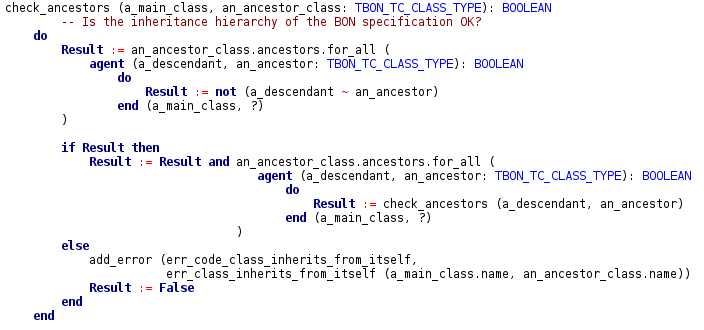
\includegraphics[scale=0.7]{images/check_ancestors_eiffel_code.png}
}
\caption{Eiffel implementation of the \textit{check}\textunderscore\textit{ancestors} algorithm}
\label{fig:eiffel_check_ancestors}
\end{figure}

\paragraph{}
In figure \ref{fig:eiffel_check_ancestors} the actual implementation in Eiffel is shown. The most notable difference between the implementation and the pseudocode is that when the it is iterating through the ancestors to call \textit{check}\textunderscore\textit{ancestors} on the ancestors, it is \textbf{and}'ed with \textbf{Result}. This does not change how the program works, due to the conditional statement ensuring that \textbf{Result} always is \textbf{True} at that point. It is done to express that the value of \textbf{Result} does not only depend on the returned value of the expression, but also on the previous evaluation of the direct ancestors. This means that the conditional statement could have been excluded, but as it stops the algorithm from further unnecessary iterations when a type error has been found, it is included.

Lastly, the error handling is done by the type checker's error handling section. This will be further described in section \ref{implementation-error-handling}.
\import{./}{implementation-informal-bon}

\import{./}{implementation-formal-bon}

\subsection{Error handling}
\label{implementation-error-handling}